\documentclass[12pt,a4paper,english]{article}
\usepackage{times}
\usepackage[utf8]{inputenc}
\usepackage{babel,textcomp}
\usepackage{mathpazo}
\usepackage{mathtools}
\usepackage{amsmath,amssymb}
\usepackage{ dsfont }
\usepackage{listings}
\usepackage{graphicx}
\usepackage{ mathrsfs }
\usepackage{float}
\usepackage{subfig} 
\usepackage[colorlinks]{hyperref}
\usepackage[usenames,dvipsnames,svgnames,table]{xcolor}
\usepackage{textcomp}
\definecolor{listinggray}{gray}{0.9}
\definecolor{lbcolor}{rgb}{0.9,0.9,0.9}
\lstset{backgroundcolor=\color{lbcolor},tabsize=4,rulecolor=,language=python,basicstyle=\scriptsize,upquote=true,aboveskip={1.5\baselineskip},columns=fixed,numbers=left,showstringspaces=false,extendedchars=true,breaklines=true,
prebreak=\raisebox{0ex}[0ex][0ex]{\ensuremath{\hookleftarrow}},frame=single,showtabs=false,showspaces=false,showstringspaces=false,identifierstyle=\ttfamily,keywordstyle=\color[rgb]{0,0,1},commentstyle=\color[rgb]{0.133,0.545,0.133},stringstyle=\color[rgb]{0.627,0.126,0.941},literate={å}{{\r a}}1 {Å}{{\r A}}1 {ø}{{\o}}1}

% Use for references
\usepackage[square,comma,numbers]{natbib}
%\DeclareRobustCommand{\citeext}[1]{\citeauthor{#1}~\cite{#1}}

% Fix spacing in tables and figures
%\usepackage[belowskip=0pt,aboveskip=5pt]{caption}
%\setlength{\intextsep}{10pt plus 2pt minus 2pt}

% Change the page layout
%\usepackage[showframe]{geometry}
\usepackage{layout}
\setlength{\hoffset}{-0.5in}  % Length left
\setlength{\voffset}{-0.8in}  % Length on top
\setlength{\textwidth}{470pt}  % Width /597pt
\setlength{\textheight}{670pt}  % Height /845pt
%\setlength{\footskip}{25pt}

\newcommand{\VEV}[1]{\langle#1\rangle}
\title{FYS4150 - Project 5\\
The Solar System}
\date{}
\author{ Kristoffer Langstad\\ \textit{krilangs@uio.no}}

\begin{document}
\maketitle
\begin{abstract}
	In this project we want to model the Solar System using ordinary differential equations and object orientation numerically. To do this we will use the so-called velocity Verlet algorithm. We start of with only the Earth and the Sun in the system, which we will solve with both Euler's forward algorithm and the velocity Verlet algorithm. For this simple two-body system we write the code to be object oriented and scaled with the Sun mass as $M_\odot=1$, and test the stability of the two algorithms. The Verlet algorithm is found to be superior in accuracy since the algorithm conserves the energy of the system, while the forward Euler algorithm does not. The Euler algorithm is faster, but the difference is so small that the Verlet algorithm is the best to use. Then we find properties like the escape velocity of Earth needed to escape the orbit of the Sun. This is found analytically to be $\sqrt{8}\pi\frac{\text{AU}}{\text{yr}}\approx8.88577\frac{\text{AU}}{\text{yr}}$, and numerically as $8.88250\frac{\text{AU}}{\text{yr}}$ with the velocity Verlet algorithm. By changing the gravitational force factor $\frac{1}{r^3}\rightarrow\frac{1}{r^{\beta}}$, we see that as $\beta\rightarrow4$ (for 3D) the escape velocity of the Earth escaping the Sun's orbit is decreasing more and more. So by changing the force factor, we change how strongly the orbit of the Earth is affected by the Sun. Then the system is altered to a three-body problem by introducing Jupiter to the system. First we keep the Sun as the center of mass of the system and study once again the stability of the Verlet algorithm. For 1x and 10x times the mass of Jupiter, the system is more or less stable, but when increasing the Jupiter mass by 1000 the system becomes chaotic since the Jupiter mass is around the same as the Sun mass. Now by setting the center of mass of the system as the origin of the Solar System, we add the rest of the planets (including Pluto) in the Solar System. Up till now we have used Newtonian physics, so we add a general relativistic correction to the gravitation force. This is used on the Sun-Mercury system to analyze the perihelion precession of Mercury. This observed value is found to be 43 arc seconds per century, while our numerical value is found to be 43.088 arc seconds per century.
\end{abstract}

\section{Introduction}
\label{sect:Introduction}
In many cases, like the Solar System, we have many coupled ordinary differential equations which in many ways are similar to each other. Often the only differences are constants and variables that differ them from each other. So to reduce the amount of code and to make are lives much easier for solving these equations, we can use object orientation. This makes it easy extend and to add more elements without having to add a lot of new code. The code is then rerun several times instead. This is done in this project by implementation of classes to make the code more reusable.

In this project we will solve the Solar System with ordinary differential equations with an object oriented code. The algorithms we will use are the forward Euler algorithm and the velocity Verlet algorithm. In the first part we study the two-body Sun-Earth only system to test the stability of the algorithms. Here we test the stability with different time steps and test for energy conservation in the system for the two algorithms. Then we calculate system properties like the escape velocity of Earth, and test what happens when we change the gravitational force between the objects. With the object oriented code fully set up, we can easily add other object to the system like Jupiter. The system is now a three-body system. Here we study what happens to the system when we increase the mass of Jupiter. Then we extend to include all the planets in the Solar System (including Pluto), which is easily done by adding masses and initial conditions of the planets and running the classes more times. The initial conditions of the Sun and the planets are found at a site by NASA \cite{horizon}, which contains data like the masses, initial positions and initial velocities of the objects up to three dimensions. Lastly we study the perihelion precession of Mercury by introducing a general relativistic correction to our Newtonian gravitational force, for a system containing only the Sun and Mercury.

In the methods section we look at the theory and implementation of the algorithms and of the physics connected to our problem necessary for us to solve the ordinary differential equations and properties for the planets. This includes topics like unit scaling, derivation of the numerics, the equations for energy and angular momentum and the escape velocity, and perihelion precession of Mercury. In the results section we will look at and analyze the results we get from the methods section. Here we will discuss the results and compare with analytically found results for verification of our numerics. Last in the conclusion section, we give an overall conclusion of the results of the project we have gotten, and possible future tasks that can be done.

\section{Methods}
\label{sect:Method}
\subsection{Useful Constants}
\label{subsect:constants}
For this project we use astronomical units (AU), which is the average distance between the Sun and Earth, 1 AU = $1.5\cdot10^{11}$m. We will also use years instead of seconds, since this fits the evolution of the Solar System better. The mass of the Sun is given as $M_{\text{Sun}}=M_{\odot}=2\cdot10^{30}$kg. In Table \ref{tab:planets} we see the masses of the planets in the Solar System, including Pluto, and their respective distances to the Sun. NASA provides a web site which gives us the initial positions and initial velocities of the objects in the Solar System \cite{horizon}. These are extracted by setting type to \textit{VECTOR}, and choose the wanted planets and coordinate origin. The positions are in units of AU, while the velocities are in units of AU per day which we will change to AU per year. Since the mass of the Sun is so much larger than the planets, we will scale the masses of the planets with the mass of the Sun. These constants are implemented in the \textit{planetsLib.h}-file in the GitHub repository \ref{sect:appendix} in three dimensions.

\begin{table}[htbp]
	\centering
	%\hspace{-1cm}
	\begin{tabular}{ |c|c|c| }
		\hline \rule{0pt}{13pt}
		Planet & Mass [kg] & Distance to the Sun [AU] \\
		\hline \rule{0pt}{13pt}
		Mercury & $M_{\text{Mercury}}=3.3\cdot10^{23}$ & 0.39  \\
		\hline \rule{0pt}{13pt}
		Venus & $M_{\text{Venus}}=4.9\cdot10^{24}$ & 0.72 \\
		\hline \rule{0pt}{13pt}
		Earth & $M_{\text{Earth}}=6\cdot10^{23}$ & 1.00 \\
		\hline \rule{0pt}{13pt}
		Mars & $M_{\text{Mars}}=6.6\cdot10^{23}$ & 1.52 \\
		\hline \rule{0pt}{13pt}
		Jupiter & $M_{\text{Jupiter}}=1.9\cdot10^{27}$ & 5.20 \\
		\hline \rule{0pt}{13pt}
		Saturn & $M_{\text{Saturn}}=5.5\cdot10^{26}$ & 9.54 \\
		\hline \rule{0pt}{13pt}
		Uranus & $M_{\text{Uranus}}=8.8\cdot10^{25}$ & 19.19 \\
		\hline \rule{0pt}{13pt}
		Neptune & $M_{\text{Neptune}}=1.03\cdot10^{26}$ & 30.06 \\
		\hline \rule{0pt}{13pt}
		Pluto & $M_{\text{Pluto}}=1.31\cdot10^{22}$ & 39.53 \\
		\hline 
	\end{tabular}	
	\caption{In this table we see the masses of the planets in the Solar System with units kg, including Pluto, and their respective distances to the Sun in units AU.}
	\label{tab:planets}
\end{table}

\subsection{Newton's Law of Motion}
\label{subsect:Newton}
We will look at the gravitational force between the objects in the Solar System. This is given by Newton's law of gravitation between two objects with masses $M$ by
\begin{equation}
\label{eq:2D_FG}
F_G=\frac{GM_1M_2}{r^2},
\end{equation}
where $G=6.67\cdot10^{-11} \ \textrm{N} \ \textrm{kg}^{-2} \textrm{m}^2$ is the gravitational constant and $r$ is the distance between the objects. In three dimensions of the Solar System we get
\begin{equation}
\label{eq:3D_FG}
\textbf{F}_G=\frac{GM_1M_2}{r^3}\textbf{r},
\end{equation}
where \textbf{r} is a three-dimensional position vector in Cartesian coordinates and $r=\sqrt{x^2+y^2+z^2}$.

Newton's second law of motion in three-dimensions give that 
\begin{equation}
\label{eq:N2L}
\textbf{F}=M\textbf{a},
\end{equation}

where $M$ is the mass og the object affected by the force and \textbf{a} is a three-dimensional acceleration vector. This gives us three differential equations, one for each coordinate:
\begin{align*}
F_{G,x}&=M\frac{d^2x}{dt^2}\\
F_{G,y}&=M\frac{d^2y}{dt^2}\\
F_{G,z}&=M\frac{d^2z}{dt^2}
\end{align*}

For a two-body system with Earth orbiting around the Sun in a circular motion, the acceleration of the Earth is given by the centripetal acceleration \[a=\frac{v^2}{r}.\]
Newton's second law now yields
\begin{equation}
F_G=\frac{M_{\text{Earth}}v^2}{r}=\frac{GM_{\odot}M_{\text{Earth}}}{r^2},
\end{equation}
where $M_{\odot}$ is the mass of the Sun and $M_{\text{Earth}}$ is the mass of the Earth. By rearranging the above equation we find the following relation:
\begin{equation}
\label{eq:consts}
v^2r=GM_{\odot}
\end{equation}
We now scale the equations to simplify the calculations.
Since the motion of Earth is circular at a distance $r=1AU$ to the Sun, we use that the velocity can be written as
\begin{equation}
\label{eq:circ_vel}
v=\frac{2\pi r}{1yr}=2\pi\frac{1AU}{1yr}.
\end{equation}
By inserting this velocity into \ref{eq:consts} and redefine the mass of the Sun to $M_{\odot}=1$, we get a scaled gravitational constant as
\begin{equation}
\label{eq:scaled_G}
G=4\pi^2\frac{AU^3}{yr^2}.
\end{equation}

\subsection{Integration Methods}
\label{subsect:Integration}
In this project we use the forward Euler algorithm and the velocity Verlet algorithm. The forward Euler algorithm is a first order approximation to a differential equation solution with a local error proportional to the step size squared $\mathcal{O}(h^2)$. For a three-dimensional case, the forward Euler algorithm with $n$ points on discrete form is given as:
\begin{align}
\label{eq:1D_Euler}
\textbf{x}_{i+1}&=\textbf{x}_i+\textbf{v}_ih\\
\textbf{v}_{i+1}&=\textbf{v}_i+\textbf{a}_ih
\end{align}
For three-dimensions we have $\textbf{x}=(x,y,z)$, $\textbf{v}=(v_x,v_y,v_z)$ and $\textbf{a}=(a_x,a_y,a_z)$. Here $h=\frac{b-a}{n}$ is the step size in a domain $t\in[a,b]$, $v_i$ is the velocity, $a_i$ is the acceleration and $x_i$ is the position after $n$ steps. So by knowing the acceleration, initial positions and velocities, we can compute the position of the system. For the number of floating points (FLOPs) required to calculate the acceleration we need 19 FLOPs for three dimensions which is calculated $n(n-1)$ times. For the main forward Euler scheme in three dimensions we need 6 FLOPs for the position and 6 FLOPs for the velocity per time step. Total number of FLOPs for $n$ time steps with the forward Euler algorithm is then:
\begin{equation}
\label{eq:FLOPS_Euler}
19n(n-1)+12n=19n^2-7n
\end{equation}

The velocity Verlet algorithm has a higher order of accuracy where the local error is proportional to the step size cubed $\mathcal{O}(h^3)$. So the Verlet algorithm has a higher order accuracy than the Euler algorithm. For a three-dimensional case the velocity Verlet on discrete form is given as:
\begin{align}
\label{eq:2D_Verlet}
\textbf{x}_{i+1}&=\textbf{x}_i+\textbf{v}_ih+\frac{1}{2}\textbf{a}_ih^2\\
\textbf{v}_{i+1}&=\textbf{v}_i+\frac{1}{2}(\textbf{a}_{i+1}+\textbf{a}_i)h
\end{align}
In this case we have to calculate $\textbf{x}_i{+1}$ first, since the term $\textbf{a}_{i+1}=\textbf{a}(\textbf{x}_{i+1},t_{i+1})$ is dependent on $\textbf{x}_{i+1}$. As for the Euler scheme we need 19 FLOPs to calculate the acceleration, since we use the same calculation for the acceleration in both algorithms. For the position with Verlet in three dimensions we need 21 FLOPs and 12 FLOPs for the velocity per time step. Total number of FLOPs for $n$ number of time steps with the velocity Verlet algorithm is then:
\begin{equation}
\label{eq:FLOPS_Verlet}
19n(n-1)+33n=19n^2+14n
\end{equation}
From the calculations for the number of FLOPs in equation \ref{eq:FLOPS_Euler} and \ref{eq:FLOPS_Verlet}, we see that the Verlet algorithm requires more FLOPs, which means that the Verlet algorithm should use longer CPU time.

\subsection{Energies}
\label{subsect:Energies}
Since the gravitational force is conservative, the total energy of the system should be constant over time. This is one of the stability criteria of our algorithms. The total energy of the system is given by the sum of kinetic energy and potential energy $E=K+U$. The total kinetic energy of the system with $N$ objects is given as
\begin{equation}
\label{eq:K}
K=\sum_{i=1}^{N}\frac{1}{2}M_iv_i^2,
\end{equation}
where $M_i$ is the mass and $v_i$ is the velocity of object $i$. The total potential energy of the system is given as 
\begin{equation}
\label{eq:U}
U=\sum_{i=1}^{N}\sum_{j+1}^{N}\frac{GM_iM_j}{r_{j,i}},
\end{equation}
where $i$ and $j$ are summing over different objects and $r_{j,i}=|\textbf{r}_i-\textbf{r}_j|$.

\subsection{Angular Momentum}
\label{subsect:Ang_mom}
The angular momentum describes the rotational state of the system. Since there is no external forces acting on the system, then also the total angular momentum of the system should be constant over time in our Solar System. The total angular momentum is given as
\begin{equation}
\label{eq:ang_mom}
\textbf{L}=\sum_{i=1}^{N}M_i\textbf{r}_i\times \textbf{v}_i.
\end{equation}

\subsection{Testing the Algorithms}
\label{subsect:Testing}
With the algorithms implemented into a program and the initial velocity value giving circular orbit from equation \ref{eq:circ_vel} as $v=2\pi$, we plot the position of the Earth orbiting the Sun. Here we test the two algorithms by first using different time steps $\Delta t$ when plotting the position of the Earth. For the case with circular orbit, we study the kinetic and potential energies and the angular momentum of the system. These quantities should be conserved over time as explained earlier. We also do a timing of the algorithms to compare with each other. Here we expect the Verlet algorithm to use longer CPU time than the Euler algorithm (see section \ref{subsect:Integration}). From these calculations we compare the different results we get by using the Euler algorithm versus using the Verlet algorithm, and discuss the differences of the two methods. For the rest of the project we will use the Verlet algorithm.

\subsection{Escape Velocity}
\label{subsect:Escape vel}
For an object in orbit around a more massive orbit, say the Earth around the Sun, to escape out of the orbit, it have to have a specific minimum velocity. This velocity is called the escape velocity. This is found from energy conservation by using that the kinetic energy is equal to the potential energy. So by using the kinetic energy in equation \ref{eq:K} and the potential energy in equation \ref{eq:U}, we obtain the escape velocity as
\begin{equation}
\label{eq:v_esc}
v_{esc}=\sqrt{\frac{2GM}{r}},
\end{equation}
where $M$ is the mass of the body the object is trying to escape from and $r$ is the distance to that body. If we consider the Earth at a distance $r=1$ AU from the Sun with mass $M_{\odot}=1$ and use the scaled gravitational constant in equation \ref{eq:scaled_G}, we obtain the escape velocity of Earth as 
\begin{equation}
\label{eq:v_esc_Earth}
v_{esc}=\sqrt{8}\pi\frac{AU}{yr}.
\end{equation}
We calculate the escape velocity of the Earth numerically and compare with the analytic answer we just derived in equation \ref{eq:v_esc_Earth}.

Then we try to change the gravitational force in equation \ref{eq:3D_FG} to 
\begin{equation}
\label{eq:change_beta}
F_G=\frac{GM_{\odot}M_{\text{Earth}}}{r^{\beta}},
\end{equation}
where we change $\beta\in[3,4]$ (for three-dimensions) to see what happens to the Earth-Sun system when $\beta\rightarrow4$.

\subsection{Three-Body Problem}
\label{subsect:Add Jupiter}
Now we will add Jupiter such that we now have a three-body problem with the Sun fixed at the center of mass of the system. Now we want to check how adding Jupiter will change the Earth's motion. To do this we just add the magnitude of the force between the Earth and Jupiter as
\begin{equation}
\label{eq:Earth-Jupiter}
F_{E-J}=\frac{GM_EM_J}{r^3_{E-J}},
\end{equation}
where $M_J$ is the mass of Jupiter, $M_E$ is the mass of the Earth and $r_{E-J}$ is the distance between Earth and Jupiter (here in 3D). Since we have a object oriented code with classes, it is easy to implement Jupiter into the calculation of the motion of the planets in the three-body system. So now we plot the position of the Earth and Jupiter using the Verlet algorithm. We also do the same for increasing the mass of Jupiter by 10 and 1000 times its initial mass, to see what happens to the system.

\subsection{The Whole Solar System}
\label{subsect:SolarSystem}
We will now change the center of mass to the origin instead of at the Sun (still very close to the Sun). Now the Sun will also have an initial velocity such that the total momentum of the system is zero. With this change of mass center we can compare with the other three-body problem to see that difference to the system.

We now also add the rest of the planets in the Solar System, including Pluto. Their masses and initial conditions are implemented as mentioned in the earlier section (\ref{subsect:constants}), and then we plot the whole Solar System.

\subsection{Perihelion of Mercury}
\label{subsect:Mercury}
Finally we will test general relativity by comparing the perihelion precession of Mercury to the observed value. Closed elliptical orbits comes from the Newtonian gravity force factor $1/r^2$. By changing this factor, we change the orbit to no longer being closed. This means that after one complete orbit around the Sun, the planet will not be in the exactly same place as before. Mercury has an observed perihelion precession of 43 arc seconds per century after the classical effects are subtracted. 

To study this we look at the Sun-Mercury system, and add a relativistic corrective term to the Newtonian gravitational force such that we obtain
\begin{equation}
\label{eq:rel_FG}
F_G=\frac{GM_{\odot}M_{\text{Mercury}}}{r^2}\left[1+\frac{3l^2}{r^2c^2}\right],
\end{equation} 
where $r$ is the distance between the Sun and Mercury, $c$ is the speed of light in vacuum in units AU/yr and $l=|\textbf{r}\times \textbf{v}|$ is the magnitude of Mercury's orbital angular momentum per unit mass. We want to study the perihelion angle $\theta_p$ over one century around the Sun with \[\tan\theta_p=\frac{y_p}{x_p},\] where $x_p$ and $y_p$ are the $x$ and $y$ positions of Mercury at perihelion, which is the position when Mercury is closest to the Sun. We will use that the speed of Mercury at perihelion is 12.44 AU/yr with the perihelion at a distance of 0.3075 AU from the Sun.

\subsection{Implementation}
\label{subsect:Implementation}
The main code is done in C++ in Qt Creator on a Windows 10 computer with the following terminal command: \[\textit{c++ -floop-parallelize-all -o main.exe main.cpp classes.cpp utils.cpp SolarSystem.cpp}\]
We also use the \textit{-Ofast} compiler flag to increase the speed. All the C++ programs can be found in the Codes folder at the GitHub repository \ref{sect:appendix}.

In this project we want to use object orientation to easily extend our programs without having to write much more code. We do this by using classes, which means that we can reuse much of the code. We write a main class for using the Euler and Verlet algorithms to simulate the positions and velocities of the planets in the Solar System. This class \textbf{Obj} is implemented in the \textit{classes.cpp} program. This class also sets initial conditions, gets the acceleration and velocities of objects, times the algorithms and inherits functions from another program to among others to write results to text files extracted to a Data folder. The program the class inherits from is the \textit{utils.cpp}, here we have supporting functions for creating vectors, matrices and writing to text files. These functions do not work alone and have to be imported by other classes or programs. In the \textit{SolarSystem.cpp} program we have to other classes; the \textbf{SolarSystem} class is a subclass of \textbf{Obj} and calculates the acceleration, energies and angular momentum of the objects. The other class is the \textbf{SolarRelativistic} class which is a subclass of \textbf{SolarSystem} and calculates the perihelion precession of Mercury by using modified Verlet algorithm with the relativistic gravity term. In the \textit{main.cpp} program, we do the main calculation for simulating the Solar System by setting the variable values to by used by the various classes and functions mentioned above.

For the plotting we use Python 3.7 in Spyder, and all the figures are stored in a folder \textit{Figures} as in the GitHub repository \ref{sect:appendix}. The Python program extracts the data from the data files in the Data folder, and plots the wanted figures.

\section{Results}
\label{sect:Results}
The first thing we do is to test the two algorithms. We first look at the stability in the two algorithms by plotting the motion of the Earth around the Sun with different time steps $\Delta t\in[0.1,1e-5]$. In Figure \ref{fig:EulerVsVerlet} we see the motion of the Earth around the Sun with $\Delta t=0.001$ for both the forward Euler and the velocity Verlet algorithms. For the Euler plot we see that the orbit changes for each round around the Sun. For the other plots with other time steps, see the Figures folder at the GitHub repository \ref{sect:appendix}. In these plots we see that for $\Delta t=0.1$ both the algorithms give pretty bad orbits, Euler doesn't even complete one round around the Sun. As $\Delta t\rightarrow 1e-5$, the motion of the Earth with the Verlet algorithm quickly becomes quite good. With the Euler algorithm, the motion of Earth does not become satisfactory until $\Delta t=1e-5$. From this analysis we clearly see that the Verlet algorithm is superior in accuracy much quicker than the Euler algorithm.

\begin{figure}[htbp]
	%\hspace*{-2.5cm}
	\subfloat[Motion of the Earth around the Sun with the forward Euler algorithm. \label{fig:Euler} ]{\includegraphics[width=0.5\linewidth]{earth_sun_euler_0_001.png}}
	\hspace{0.5em}
	\subfloat[Motion of the Earth around the Sun with the velocity Verlet algorithm. \label{fig:Verlet} ]{\includegraphics[width=0.5\linewidth]{earth_sun_verlet_0_001.png}}
	\caption{Here we see plots of the motion of the Earth around the Sun with time step $\Delta t=0.001$ with the forward Euler algorithm (\ref{fig:Euler}) and the velocity Verlet algorithm (\ref{fig:Verlet}). Here we see that the Verlet algorithm keeps the same orbit, while with Euler the orbit changes with time.\label{fig:EulerVsVerlet}}
\end{figure}

Another thing to look at in case of stability of the algorithms, is that the energies and angular momentum is conserved with the algorithms as explained in the Energies (\ref{subsect:Energies}) and Angular Momentum (\ref{subsect:Ang_mom}) sections. In Figure \ref{fig:Energies} we see the kinetic, potential and total energies of the Earth with $\Delta t=0.001$ with the Euler and Verlet algorithm. From these plots we see that with the Verlet algorithm the energies are constant/conserved as time increases. For the Euler algorithm we see that the energies change as time increases. In Figure \ref{fig:Angular} we see the angular momentum of the Earth for $\Delta t=0.001$ for the Euler and Verlet algorithms. From these plots we see that the angular momentum with the Verlet is conserved, while again it is not with the Euler algorithm. So we can conclude that the velocity Verlet algorithm is the best of the two to use here since it conserves both the energies and the angular momentum.

\begin{figure}[htbp]
	%\hspace*{-2.5cm}
	\subfloat[Kinetic, potential and total energy with the forward Euler algorithm. \label{fig:Euler_Energy} ]{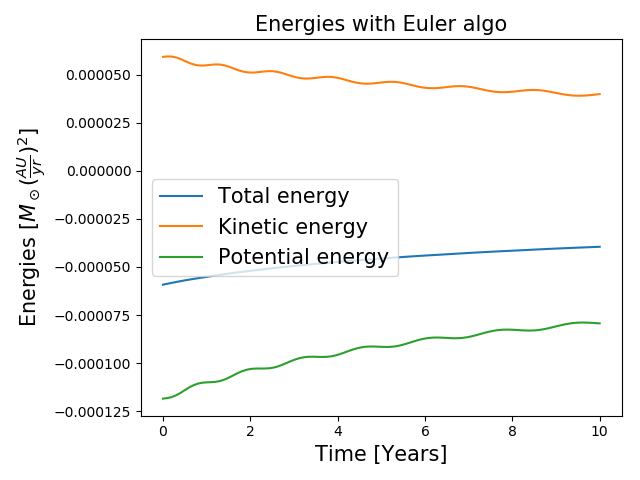
\includegraphics[width=0.5\linewidth]{Energy_earth_sun_euler_1000.png}}
	\hspace{0.5em}
	\subfloat[Kinetic, potential and total energy with the velocity Verlet algorithm. \label{fig:Verlet_Energy} ]{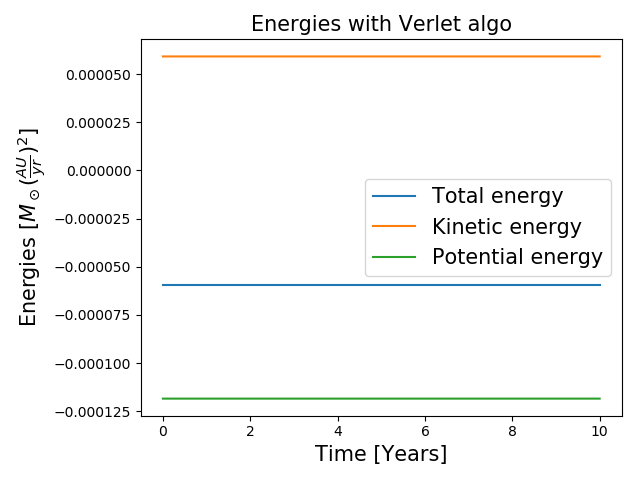
\includegraphics[width=0.5\linewidth]{Energy_earth_sun_verlet_1000.png}}
	\caption{Here we see plots of the kinetic, potential and total energy for $\Delta t=0.001$ with the Euler and Verlet algorithms. Here we see that with the Verlet algorithm, the energies are conserved as time increases. This is not the case with the Euler algorithm. \label{fig:Energies}}
\end{figure}

\begin{figure}[htbp]
	%\hspace*{-2.5cm}
	\subfloat[Kinetic, potential and total energy with the forward Euler algorithm. \label{fig:Euler_Angular} ]{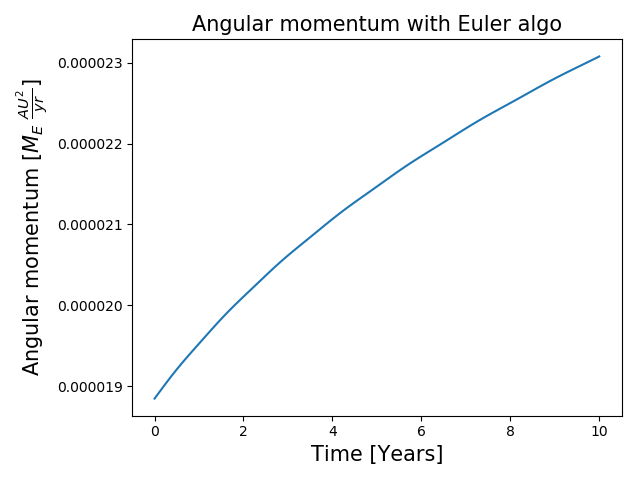
\includegraphics[width=0.5\linewidth]{Mom_earth_sun_euler_1000.png}}
	\hspace{0.5em}
	\subfloat[Angular momentum with the velocity Verlet algorithm. \label{fig:Verlet_Angular} ]{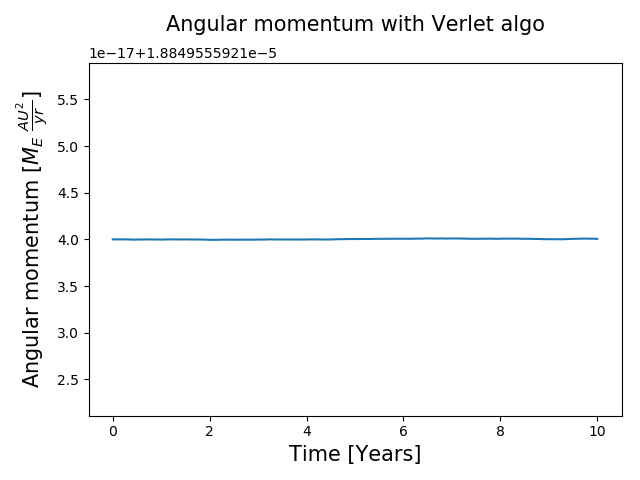
\includegraphics[width=0.5\linewidth]{Mom_earth_sun_verlet_1000.png}}
	\caption{Here we see plots of the angular momentum for $\Delta t=0.001$ with the Euler and Verlet algorithms. Here we see that with the Verlet algorithm, the angular momentum is conserved as time increases. This is not the case with the Euler algorithm as for the energies. \label{fig:Angular}}
\end{figure}

From the number of FLOPs with the algorithms discussed in the Integration methods section (\ref{subsect:Integration}), we expect the Euler algorithm to be faster than the Verlet. In Table \ref{tab:times} we have the CPU run times of the algorithms with varying time steps taken as averages after a few runs. From this table we see that the Euler algorithm is barely faster than the Verlet algorithm. Thus, since the CPU time difference between the algorithms is not noticeable and that the Verlet algorithm conserves the energies and angular momentum, the velocity Verlet algorithm is the preferred algorithm to use further.

\begin{table}[htbp]
	\centering
	%\hspace{-1cm}
	\begin{tabular}{ |c|c|c| }
		\hline \rule{0pt}{13pt}
		n & Forward Euler [s] & Velocity Verlet [s] \\
		\hline \rule{0pt}{13pt}
		$10^3$ & 0.000999 & 0.000997  \\
		\hline \rule{0pt}{13pt}
		$10^4$ & 0.010971 & 0.011004 \\
		\hline \rule{0pt}{13pt}
		$10^5$ & 0.104720 & 0.114698 \\
		\hline \rule{0pt}{13pt}
		$10^6$ & 1.036199 & 1.127986 \\
		\hline \rule{0pt}{13pt}
		$10^7$ & 10.693399 & 11.334689 \\
		\hline 
	\end{tabular}	
	\caption{In this table we see the average CPU times in seconds of the forward Euler algorithm and the velocity Verlet algorithm. Here we see that the Euler algorithms is just faster than the Verlet algorithm. Since the Verlet has a better accuracy and the difference in times are so small, the Verlet seems to be the superior of the two.}
	\label{tab:times}
\end{table}

For the escape velocity of the Earth to escape the orbit around the Sun we test first different initial velocities. This velocity we was also found both analytically, in the Escape Velocity section (\ref{subsect:Escape vel}), and numerically. So since we know analytically what the escape velocity should be, $v_e=\sqrt{8}\pi$ AU/yr, we test different initial velocities around this value. In Figure \ref{fig:escape_vel} we have plotted the orbit of the Earth around the Sun for initial velocities just above and below the analytical escape velocity. For velocity just below the escape velocity we get a still circular orbit which goes far away from the Sun in the x-direction. For velocity just above, the Earth escapes the orbit around the Sun as expected. The numerically found escape velocity is $v\approx 8.88250$ AU/yr, which is very close to the analytical escape velocity $v_e\approx 8.88577$ AU/yr.

\begin{figure}[htbp]
	\centering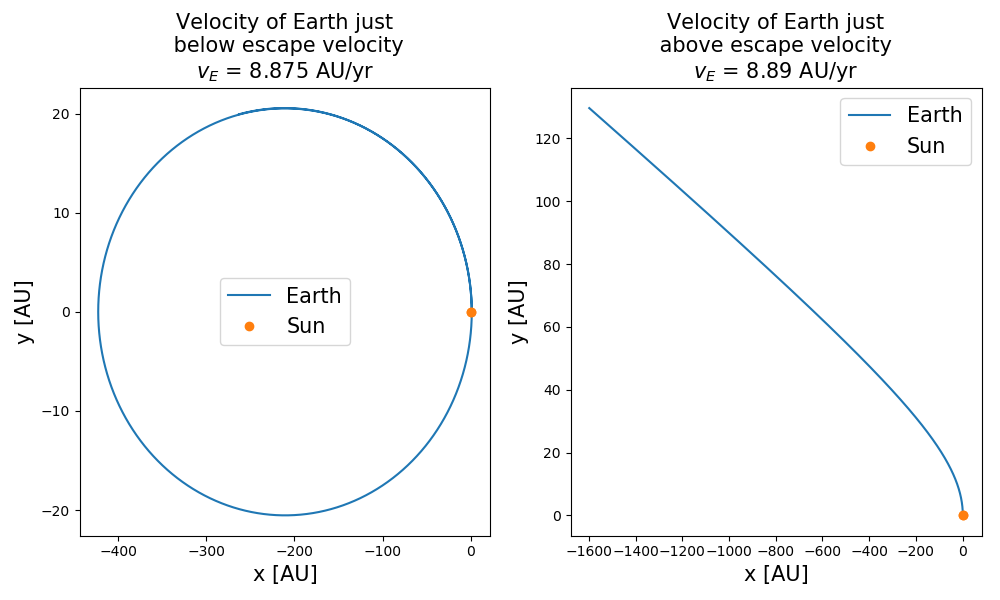
\includegraphics[width=0.8\linewidth]{Velocities_min_max.png}
	\caption{Here we see plots of the orbit of the Earth with different initial velocities, used to find the escape velocity. We have plotted for initial velocities just above and below the analytical escape velocity of $v_e=\sqrt{8}\pi$ AU/yr. For initial velocity just below the escape velocity, the orbit of the Earth is still circular but the orbit goes far away from the Sun. For initial velocity just above, the Earth escapes the orbit as expected. \label{fig:escape_vel}}
\end{figure}

Then we change the gravitational force to equation \ref{eq:change_beta} with $\beta\in[3,4]$. In Figure \ref{fig:beta_change} we see plots of the orbit of the Earth around the Sun with a chosen initial velocity $v=6.8$ AU/yr and increasing $\beta$. There we see that as $\beta\rightarrow4$, the orbit becomes more unstable and eventually the Earth escapes the Sun. So as $\beta$ increases, the escape velocity decreases. This can also be seen by looking at more figures in the Figures folder at the GitHub repository (\ref{sect:appendix}. There we also increase the initial velocity of the Earth to easier see the effect of changing $\beta$.

\begin{figure}[htbp]
	%\hspace*{-2.5cm}
	\subfloat[Orbit of the Earth around the Sun with initial veloicty $v=6.8$ AU/yr and $\beta=3.00$. \label{fig:Beta_3} ]{\includegraphics[width=0.5\linewidth]{Beta_change_3_00.png}}
	\hspace{0.5em}
	\subfloat[Orbit of the Earth around the Sun with initial veloicty $v=6.8$ AU/yr and $\beta=3.33$. \label{fig:Beta_3.33} ]{\includegraphics[width=0.5\linewidth]{Beta_change_3_33.png}}\\
	\subfloat[Orbit of the Earth around the Sun with initial veloicty $v=6.8$ AU/yr and $\beta=3.67$. \label{fig:Beta_3.67} ]{\includegraphics[width=0.5\linewidth]{Beta_change_3_67.png}}
	\hspace{0.5em}
	\subfloat[Orbit of the Earth around the Sun with initial veloicty $v=6.8$ AU/yr and $\beta=4.00$. \label{fig:Beta_4} ]{\includegraphics[width=0.5\linewidth]{Beta_change_4_00.png}}
	\caption{Here we see plots of the orbit of the Earth around the Sun with initial velocity $v=6.8$ AU/yr and varying $\beta$. As $\beta\rightarrow4$, the orbit becomes more unstable. When $\beta=4$, the Earth now escapes the orbit around the Sun. \label{fig:beta_change}}
\end{figure}

Then the system is modified to a three-body problem by introducing Jupiter. In Figure \ref{fig:PosEarthJupiter} we see the motion of the Earth and Jupiter with different masses of Jupiter for a run of 50 years. For the normal mass of Jupiter we see that the orbits are circular and smooth as expected. When increasing the Jupiter mass by a factor of 10, the orbits does not change by much (not taken with here). When we increase the mass of Jupiter by a factor of 1000, the Jupiter has a mass approximately equal to the Sun. This makes the motion of the Earth chaotic and unstable. Up until around 45 years of runtime, the Earth has a chaotic orbit around the Sun and Jupiter. After that, the Earth is thrown out of its orbit and away from the system. For the energies in Figure \ref{fig:EarthJupiterEnergies} we see that the total energy is conserved as time increases, and the only thing that changes between the mass factor change in Jupiter is the energy magnitudes. For plots for 10 times the Jupiter mass and the angular momentum see the Figures folder at the GitHub repository (\ref{sect:appendix}).

\begin{figure}[htbp]
	%\hspace*{-2.5cm}
	\subfloat[Motion of the Earth and Jupiter. \label{fig:EarthJupiter} ]{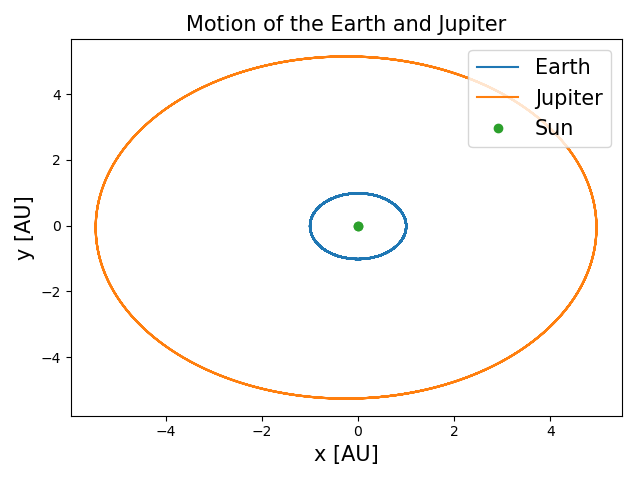
\includegraphics[width=0.5\linewidth]{EarthJupiter.png}}
	\hspace{0.5em}
	\subfloat[Motion of the Earth and Jupiter with 1000 times the Jupiter mass. \label{fig:EarthJupiter1000} ]{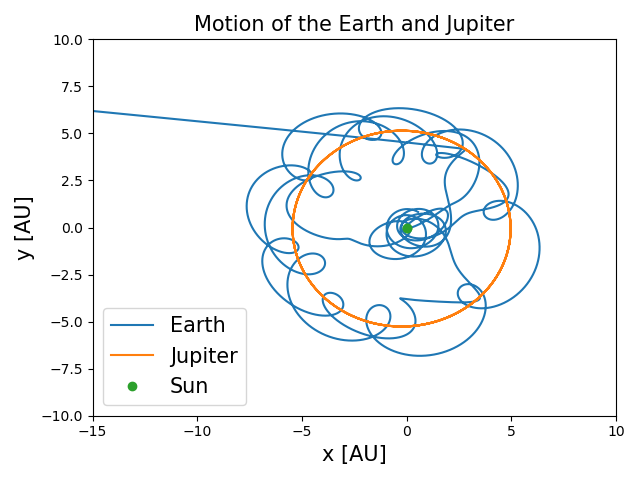
\includegraphics[width=0.5\linewidth]{EarthJupiter1000x.png}}
	\caption{Here we see plots of the motions of the Earth and Jupiter with 1x and 1000x the mass of Jupiter for 50 years. For 1x we see that the orbits are smooth and circular. When increasing the mass of Jupiter by 1000x, the orbit of the Earth becomes very unstable and after around 45 years the Earth is thrown out of orbit around the Sun. \label{fig:PosEarthJupiter}}
\end{figure}

\begin{figure}[htbp]
	%\hspace*{-2.5cm}
	\subfloat[Kinetic, potential and total energy for the Earth and Jupiter system. \label{fig:EarthJupiterEnergy} ]{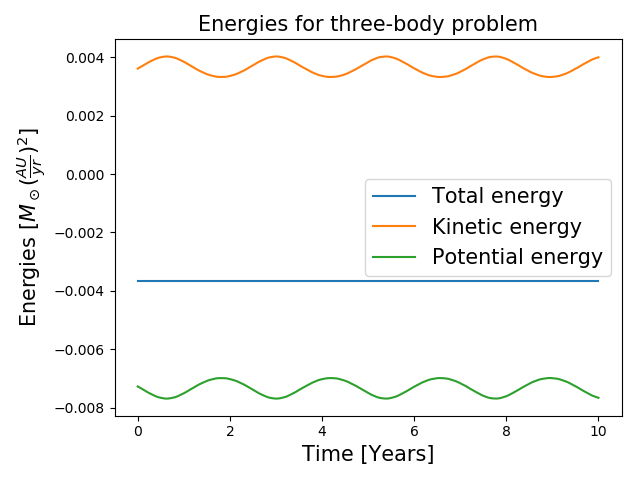
\includegraphics[width=0.5\linewidth]{Energy_EarthJupiter.png}}
	\hspace{0.5em}
	\subfloat[Kinetic, potential and total energy for the Earth and Jupiter system with 1000 times the Jupiter mass. \label{fig:EarthJupiter1000Energy} ]{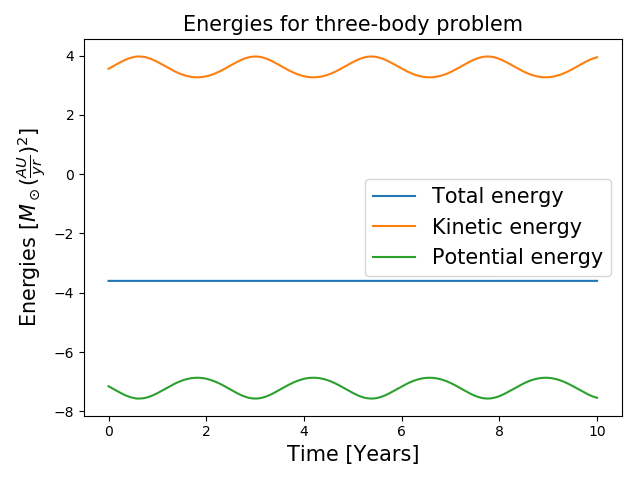
\includegraphics[width=0.5\linewidth]{Energy_EarthJupiter1000x.png}}
	\caption{Here we see plots of the kinetic, potential and total energy for the Earth and Jupiter system. Here wee see that the kinetic and potential energies very with time, but they change in such a way that the total energy is constant. Only difference between the two plots are the energy magnitudes. \label{fig:EarthJupiterEnergies}}
\end{figure}
\newpage
Now we give the Sun an initial velocity such that the total momentum of the system is zero, with the center of mass position of the three-body system as the origin. The motion of this system can be seen in Figure  \ref{fig:SunEarthJupiter}. Here we see that all the three orbits are circular and smooth. The motions in this system are close to the last system in Figure \ref{fig:EarthJupiter}, except that the Sun moves in a small circular orbit. That the Sun does not move much seems right, since the mass of the Sun is so much bigger than the other two that the mass center of the system still is within the radius of the Sun, $R_{\odot}\approx 0.00465$ AU.

\begin{figure}[htbp]
	%\hspace*{-2.5cm}
	\subfloat[Motion of the Sun, Earth and Jupiter. \label{fig:SEJ} ]{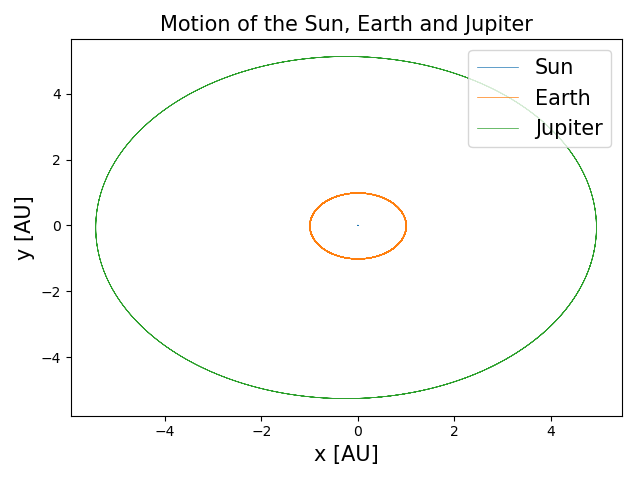
\includegraphics[width=0.5\linewidth]{SunEarthJupiter.png}}
	\hspace{0.5em}
	\subfloat[Motion of the Sun zoomed in. \label{fig:SunZoomed} ]{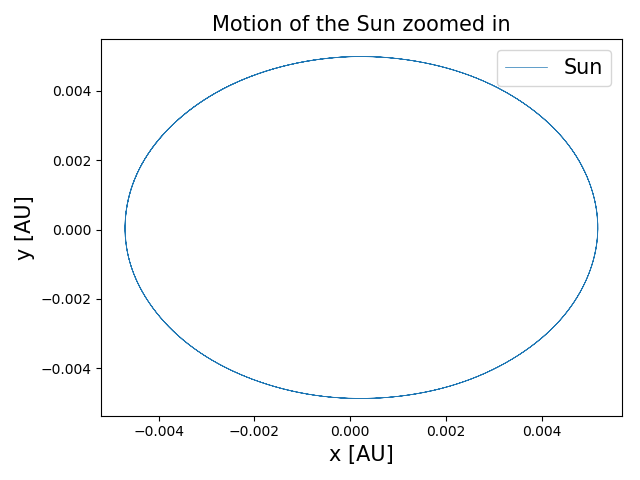
\includegraphics[width=0.5\linewidth]{SunEarthJupiter_zoomed.png}}
	\caption{Here we see plots of the motion of the new three-body system where the Sun has an initial velocity and the center of mass position is the system, and the motion of the Sun zoomed in. \label{fig:SunEarthJupiter}}
\end{figure}

Then we add the rest of the planets in the Solar System including Pluto. In Figure \ref{fig:SolarSystem} we see 2D and 3D plots of the motion of the planets in the Solar System. All the orbits are circular and smooth. Most of the planets move in a co-planar orbit around the Sun in x- and y-direction. The exception is the orbit of Pluto as seen in Figure \ref{fig:3DSolar}.

\begin{figure}[htbp]
	%\hspace*{-2.5cm}
	\subfloat[2D plot of the motion of the inner planets in the Solar System. \label{fig:2DInner_Solar} ]{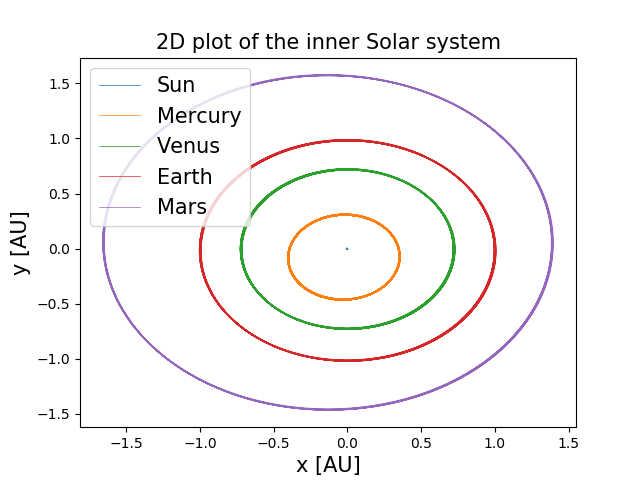
\includegraphics[width=0.55\linewidth]{2D_Inner_SolarSystem.png}}
	\hspace{0.5em}
	\subfloat[2D plot of all the planets, including Pluto, in the Solar System. \label{fig:2DSolar} ]{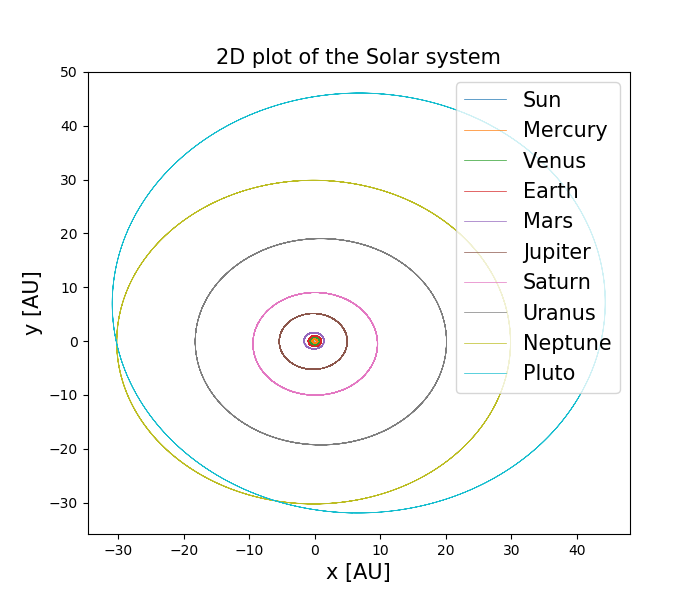
\includegraphics[width=0.5\linewidth]{2D_SolarSystem.png}}\\
	\subfloat[3D plot of all the planets, including Pluto, in the Solar System. \label{fig:3DSolar} ]{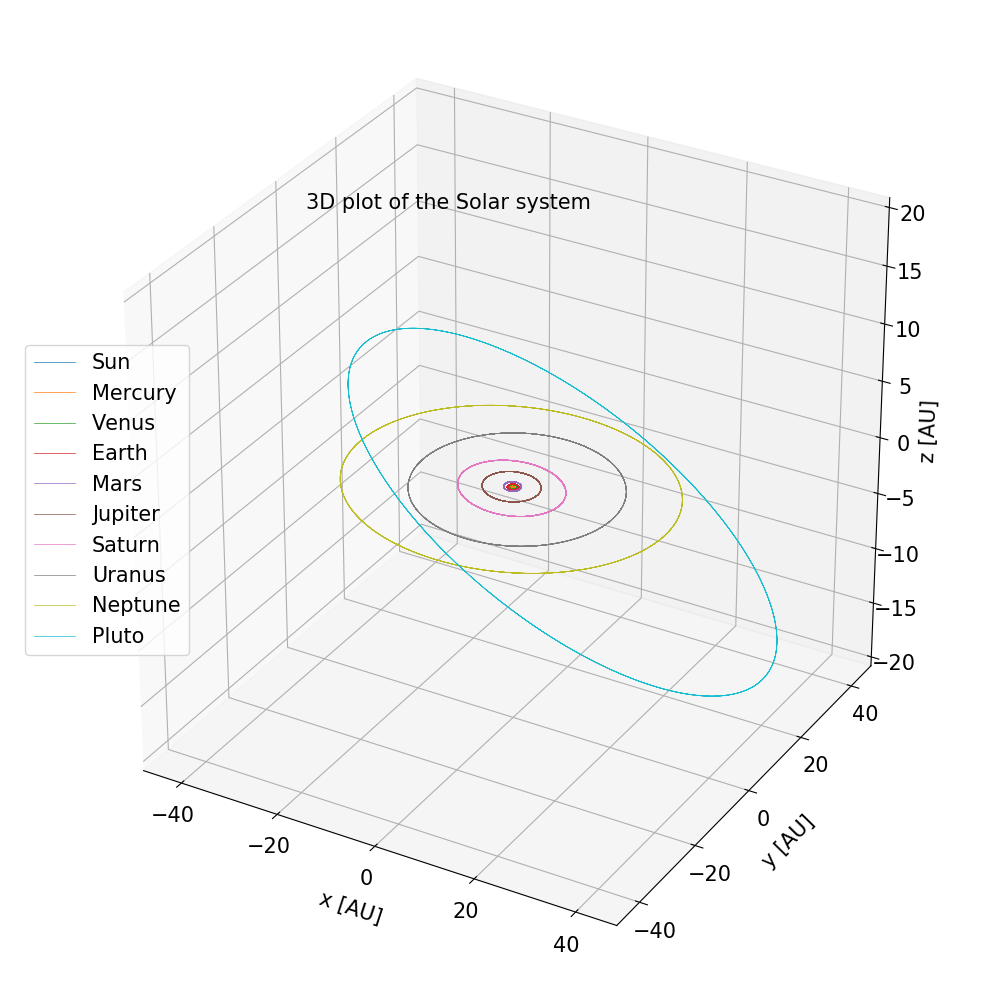
\includegraphics[width=0.7\linewidth]{3D_SolarSystem.png}}
	\caption{Plots of the Solar System in 2D and 3D. Only a 2D plot of the inner planets of the Solar System, since they are mostly co-planar. For the whole Solar System it is beneficial to plot in 3D, since the orbit of Pluto is not co-planar to the rest of the planets in x- and y-direction. \label{fig:SolarSystem}}
\end{figure}

For the perihelion precession of Mercury we add a general relativistic correction to the Newtonian gravitational force, as discussed in section \ref{subsect:Mercury}. After a century, the perihelion of Mercury should move 43 arc seconds. The numerical perihelion precession of Mercury per century we get numerically is approximately 43.088 arc seconds. So the perihelion precession of Mercury seems to be explained well with general relativity theory.

\newpage
\section{Conclusion}
\label{sect:Conclusion}
In this project we have simulated the motion of the planets in the Solar System using ordinary differential equations. To do this we have used both the forward Euler and the velocity Verlet algorithms with object orientation and scaling. 

We have tested the two algorithms by testing their stability with the Sun-Earth system. We used different time steps $\Delta t\in[0.1,1e-5]$ to simulate the orbit of the Earth around the Sun, and looked at the energy and angular momentum. From these tests we found that the Verlet algorithm is the superior since it conserved both the energies and angular momentum and gave a higher accuracy. Even though the Euler needed fewer FLOPs, the difference in CPU time between the algorithms were so small that this was negligible. That is why we used the Verlet algorithm for the rest of the project. Then we looked at the escape velocity needed for the Earth to escape the orbit around the Sun. This was found numerically by trial and error to be around 8.88250 AU/yr, which is very close to the analytical escape velocity if around 8.88577 AU/yr. Then we changed the gravitational force factor $\frac{1}{r^3}\rightarrow\frac{1}{r^{\beta}}$ to see what happened to the system when we increased $\beta$. As $\beta$ got higher, the lower the escape velocity of the Earth had to be to escape its orbit. Then we expanded to a three-body system by including Jupiter. This did not change the system much since we still had stable and smooth orbits, and the energies and angular momentum was still conserved. When we increased the mass of Jupiter to the same order as the Sun, the Verlet algorithm no longer produced reasonable results since the orbit of the Earth became chaotic. For the last expansion, the final model, we added the rest of the planets in the Solar System, including Pluto. The final model of the Solar System seemed to simulate the orbits accurate, and they seemed to be quite stable with the Verlet algorithm. Lastly we added an relativity term to the Newtonian gravitational force to test the perihelion precession of Mercury around the Sun. We got a numerically perihelion precession of around 43.088 arc seconds per century, while the observed value has been seen to be 43 arc seconds epr century. So the perihelion precession of Mercury can be explained quite well with general relativity theory.

Further work could be to implements moons around the planets in the Solar System. We could also try to improve or change the numerical algorithm for simulating the Solar System, since the used Verlet algorithm is quite good but not perfect. We could also expand the system even further, by including other solar systems to the simulation

\appendix
\section{Appendix}
\label{sect:appendix}
Link to GitHub repository:\\
\url{https://github.com/krilangs/FYS4150/tree/master/Project5}

\bibliographystyle{plainnat}
\bibliography{myrefs}
\end{document}
